% -----------------------------------------------------------------------------
% Source density.  Runs as a subsection of the growth/injury section, ahead of
% the mechanochemical part.
%
% Nothing here may redefine shared navigation state: this file is no longer
% last in the document, so any \renewcommand or \setbeamertemplate would leak
% into every section that follows it.
% -----------------------------------------------------------------------------



% % Dashed box standing in for an image that does not exist yet.
% % #1 height, #2 intended file name, #3 what the picture has to show.
% \NewDocumentCommand{\SDPlaceholder}{O{5.00cm} m m}{%
%   \begin{center}
%     \begin{tikzpicture}
%       \node[draw=HydraLine,dashed,line width=0.9pt,rounded corners=4pt,
%         inner sep=0.32cm,align=center,
%         text width=\dimexpr\linewidth-1.10cm\relax,
%         minimum height=#1]{%
%         {\color{HydraGold}\bfseries\fontsize{6.8}{8.2}\selectfont
%           FIGURE PENDING\par}
%         \vspace{0.18cm}
%         {\color{HydraWhite}\fontsize{8.0}{9.9}\selectfont #3\par}
%         \vspace{0.16cm}
%         {\color{HydraMuted}\fontsize{6.2}{7.5}\selectfont \texttt{#2}\par}
%       };
%     \end{tikzpicture}
%   \end{center}%
% }

\PerfectModel

\HydraSubsection[
  \mbox{Nothing in the equations}
  \mbox{distinguishes parts}
  \mbox{of the tissue}
]{Source density}


% Marks a slot that is filled by a simulation run live during the talk rather
% than by a static image.  Solid border, unlike \SDPlaceholder, because
% nothing is missing here.
\NewDocumentCommand{\SDLive}{O{5.00cm} m}{%
  \begin{center}
    \begin{tikzpicture}
      \node[draw=HydraCyan,line width=1.0pt,rounded corners=4pt,
        inner sep=0.32cm,align=center,
        text width=\dimexpr\linewidth-1.10cm\relax,
        minimum height=#1]{%
        {\color{HydraCyan}\bfseries\fontsize{7.4}{9}\selectfont
          LIVE SIMULATION\par}
        \vspace{0.20cm}
        {\color{HydraWhite}\fontsize{9.0}{11.4}\selectfont #2\par}
      };
    \end{tikzpicture}
  \end{center}%
}


% =============================================================================
% 2 -- The experiment, with no commentary at all.  The picture has to land on
% its own; anything written here would answer the question too early.
% =============================================================================
\begin{frame}{The same two rings, glued in two different orders}

  \vspace{-0.10cm}

  \begin{center}
    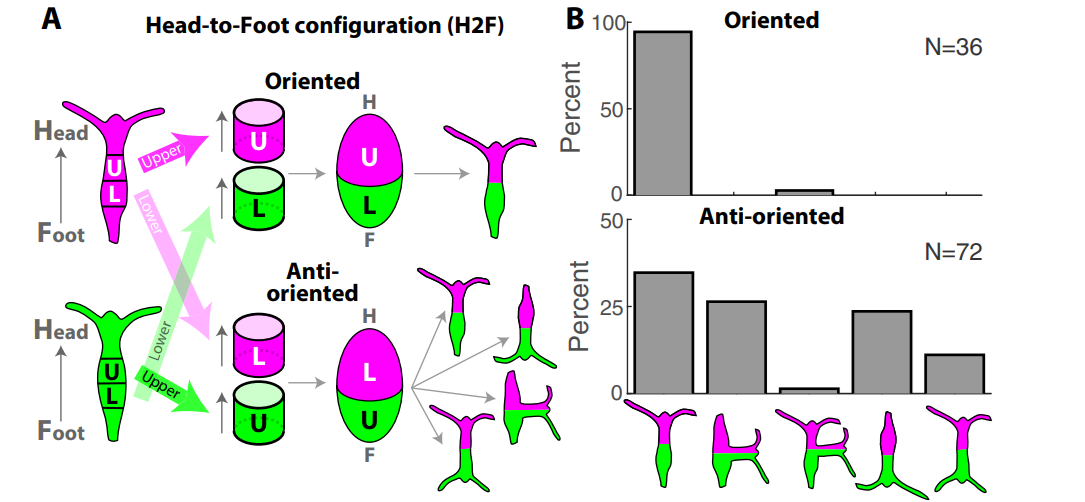
\includegraphics[
      width=0.94\textwidth,
      height=6.35cm,
      keepaspectratio
    ]{figures/Z_source_density/H2F.png}

    \vspace{0.14cm}

    {\color{HydraMuted}\fontsize{6}{7.2}\selectfont
      Livshits, Garion, Maroudas-Sacks, Shani-Zerbib, Keren \& Braun,
      \textit{Sci.\ Rep.} \textbf{12}:13368 (2022), Fig.~2A--B.\par}
  \end{center}

\end{frame}


% =============================================================================
% 3 -- Naming the missing quantity.
% =============================================================================
\begin{frame}{Missing ingredient}

  \vspace{-0.14cm}

  \begin{columns}[c,onlytextwidth]

    \begin{column}{0.40\textwidth}
      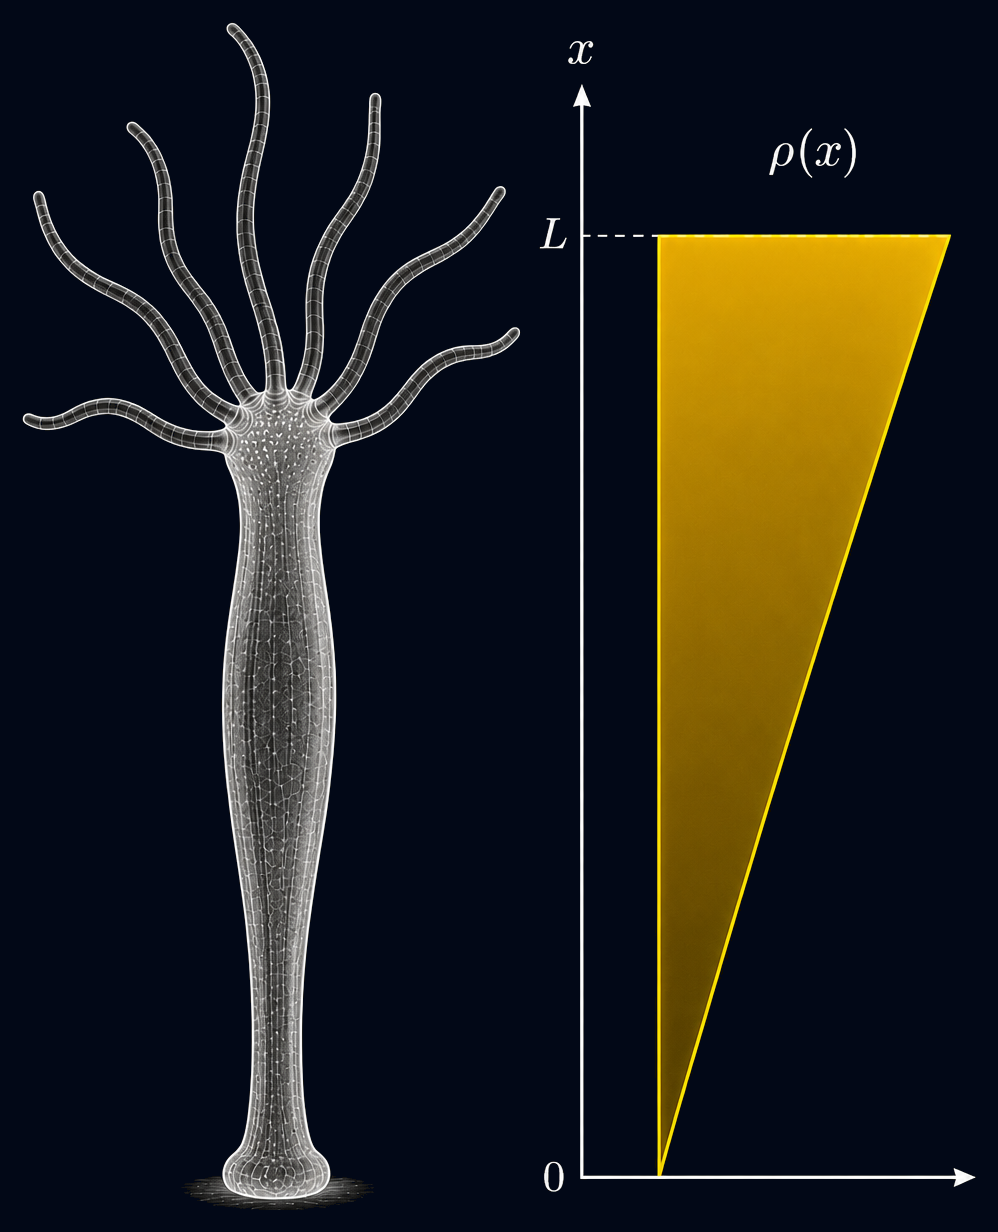
\includegraphics[
        width=\linewidth,
        height=5.45cm,
        keepaspectratio
      ]{figures/Z_source_density/rho_gradient.png}
    \end{column}

    \begin{column}{0.56\textwidth}

      \HydraPoint[HydraGold]
        {How do we tell two pieces of tissue apart?}
        {Nothing in the equations distinguishes tissue taken from near the head
         from tissue taken from near the foot.}

      \vspace{0.10cm}

      \HydraPoint[HydraCyan]
        {Positional information}
        {Each piece carries a memory of where it sat along the body axis of the
         parent animal.}

      \vspace{0.10cm}

      \HydraPoint[HydraGold]
        {$\rho(x)$ influences the production of both components}
        {The same graded factor multiplies the production of the activator and
         of the inhibitor.}

    \end{column}

  \end{columns}

\end{frame}


% =============================================================================
% 4 -- The model with rho(x).  Same numerical presentation as the model slide
% in the Gierer--Meinhardt section, so the new factor is the only difference
% the audience has to absorb.
% =============================================================================
\begin{frame}{Model with $\rho(x)$}

  \vspace{-0.30cm}

  \begin{columns}[c,onlytextwidth]

    \begin{column}{0.58\textwidth}

      {\color{HydraWhite}\fontsize{8.6}{10.6}\selectfont
      Let $\Omega=[0,1]\subset\mathbb R$ be an interval
      \par}

      \vspace{-0.34cm}

      {\color{HydraWhite}\fontsize{9.9}{12.6}\selectfont
      \begin{align*}
        \partial_tu
        &=
        0.01\Delta u
        +
        {\color{HydraGold}\rho(x)}\,
        \frac{1.5u^2}{1+v}
        -
        0.5u
        \\
        \partial_tv
        &=
        \Delta v
        +
        {\color{HydraGold}\rho(x)}\,
        2u^2
        -
        v
      \end{align*}
      }

      \vspace{-0.22cm}

      \HydraPoint[HydraCyan]
        {Initial conditions}
        {$u(x,0)=u_0(x)$ and $v(x,0)=v_0(x)$}

      \vspace{-0.14cm}

      \HydraPoint[HydraGold]
        {No-flux boundaries}
        {$\partial_x u(x,t)=\partial_x v(x,t)=0$ at $x=0$ and $x=1$}

    \end{column}

    \begin{column}{0.38\textwidth}
      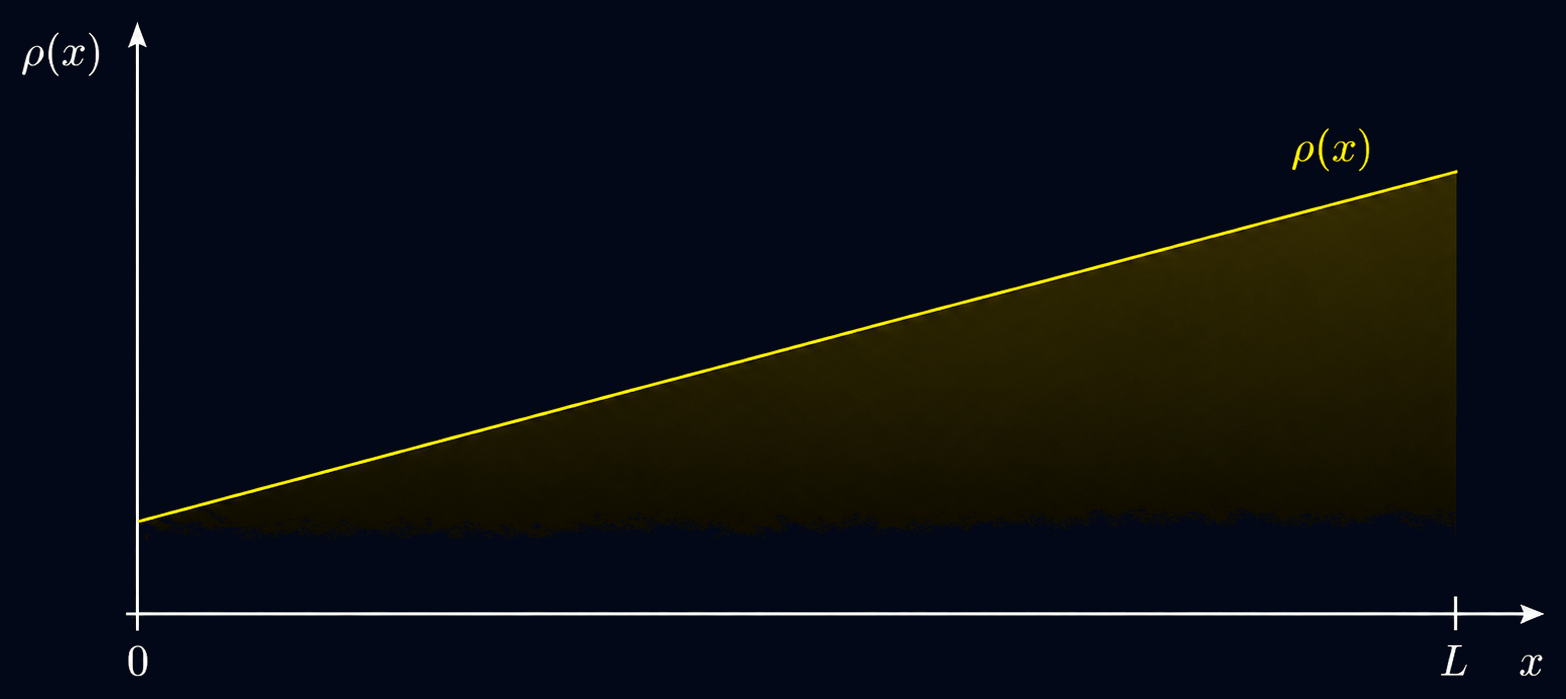
\includegraphics[
        width=\linewidth,
        height=3.30cm,
        keepaspectratio
      ]{figures/Z_source_density/rho_linear.png}
    \end{column}

  \end{columns}

  \vspace{0.24cm}

  \begin{columns}[T,onlytextwidth]

    \begin{column}{0.31\textwidth}
      {\color{HydraWhite}\bfseries\fontsize{8.0}{9.8}\selectfont
        Hard to analyse\par}
      \vspace{-0.04cm}
      {\color{HydraBody}\fontsize{6.6}{8.3}\selectfont
        A space-dependent coefficient breaks the tools built up so far.\par}
    \end{column}

    \begin{column}{0.31\textwidth}
      {\color{HydraWhite}\bfseries\fontsize{8.0}{9.8}\selectfont
        No positive constant steady state\par}
      \vspace{-0.04cm}
      {\color{HydraBody}\fontsize{6.6}{8.3}\selectfont
        Only the trivial state survives, and every earlier section
        linearised about a positive one.\par}
    \end{column}

    \begin{column}{0.31\textwidth}
      {\color{HydraWhite}\bfseries\fontsize{8.0}{9.8}\selectfont
        Theory exists, but it is heavy\par}
      \vspace{-0.04cm}
      {\color{HydraBody}\fontsize{6.6}{8.3}\selectfont
        Rigorous results are available and considerably more involved.\par}
    \end{column}

  \end{columns}

\end{frame}




% =============================================================================
% 6 -- The objection that forces the rest of the section.
% =============================================================================
\begin{frame}{But where does $\rho(x)$ come from?}

  \vspace{0.20cm}

  \HydraPoint[HydraGold]
    {It is put in by hand}
    {We chose the profile ourselves. Nothing in the model produces it.}

  \vspace{0.14cm}

  \HydraPoint[HydraCyan]
    {It never changes}
    {A prescribed $\rho(x)$ is fixed for all time, so the tissue cannot
     rewrite what it knows about its own position.}

  \vspace{0.14cm}

  \HydraPoint[HydraGold]
    {Regeneration has to restore it}
    {The animal that grows back must carry a proper gradient again, ready
     for the next cut. A prescribed profile offers no mechanism for that.}

  \vspace{0.30cm}

  \HydraTakeaway{
    If the source density matters, it has to be a variable of the model
  }

\end{frame}


% =============================================================================
% 7 -- Promoting rho to a variable.  No time scale yet: the equation relaxes
% as fast as everything else.
% =============================================================================
\begin{frame}{Source density as a variable}

  \vspace{-0.16cm}

  \begin{columns}[c,onlytextwidth]

    \begin{column}{0.46\textwidth}

      {\color{HydraWhite}\fontsize{10.2}{13}\selectfont
      \begin{align*}
        \partial_t\rho
        &=
        D_{\rho}\Delta\rho
        +
        u
        -
        \rho
      \end{align*}
      }

      \vspace{-0.20cm}

      {\color{HydraMuted}\fontsize{7.4}{9.1}\selectfont
        with $\partial_x\rho=0$ at $x=0$ and $x=1$
      \par}

      \vspace{0.34cm}

      \HydraPoint[HydraCyan]
        {The activator writes it}
        {Wherever the activator is high, the tissue becomes better at
         producing it.}

      \vspace{0.06cm}

      \HydraPoint[HydraGold]
        {Diffusion spreads it out}
        {$D_{SD}$ turns a sharp peak into a profile that varies across the
         whole domain.}

    \end{column}

    \begin{column}{0.50\textwidth}
      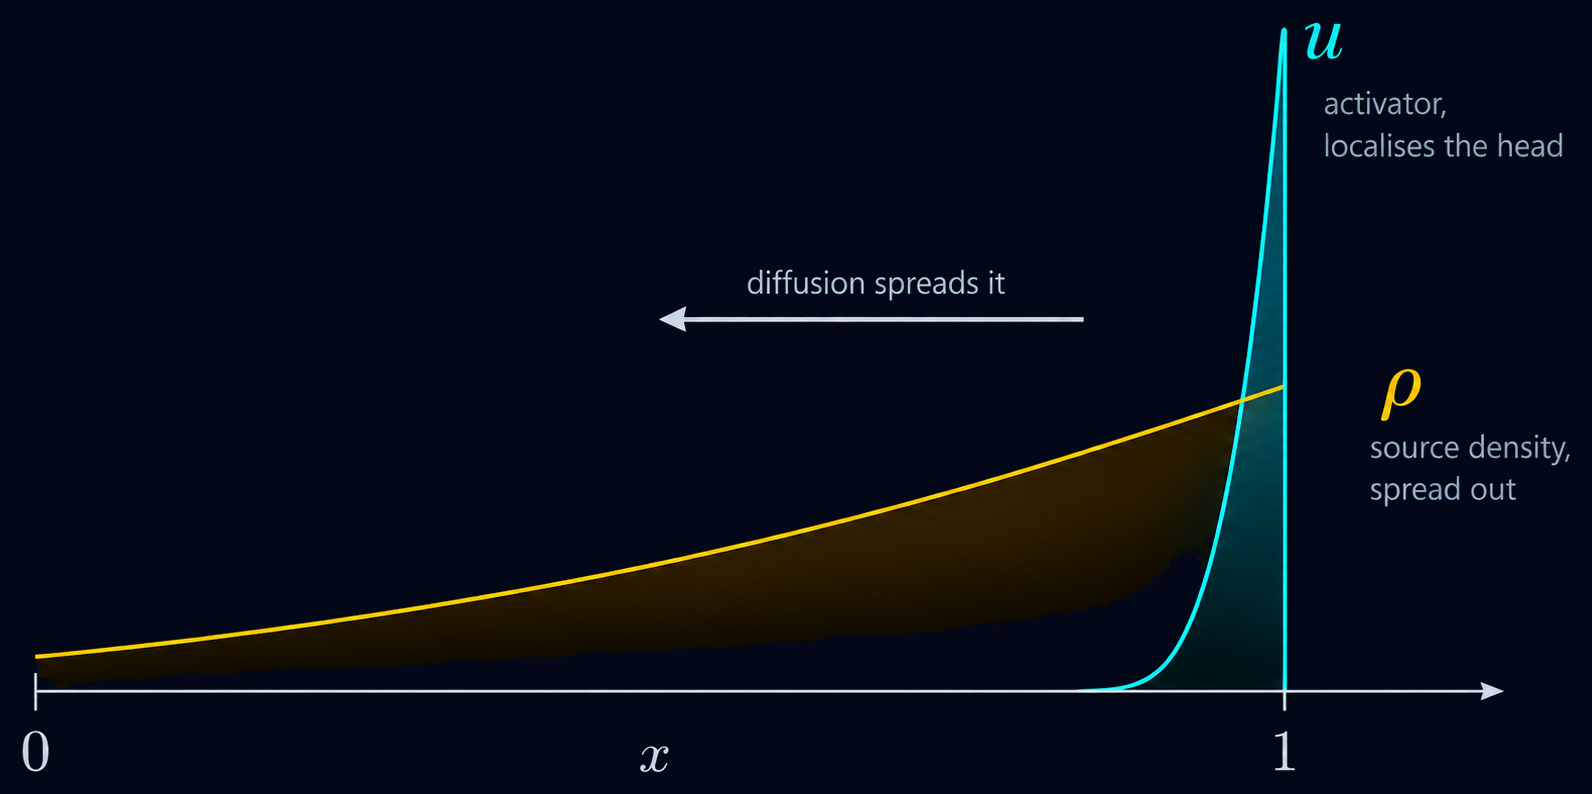
\includegraphics[
        width=\linewidth,
        height=4.75cm,
        keepaspectratio
      ]{figures/Z_source_density/rho_spreading.png}
    \end{column}

  \end{columns}

\end{frame}


% =============================================================================
% 8 -- What the analysis does and does not change.
% =============================================================================
\begin{frame}{The analysis survives, at a price}

  \vspace{-0.24cm}

  {\color{HydraWhite}\fontsize{9.7}{12.3}\selectfont
  \begin{align*}
    \partial_tu
    &=
    0.01\Delta u
    +
    \rho\,\frac{1.5u^2}{1+v}
    -
    0.5u
    \\
    \partial_tv
    &=
    \Delta v
    +
    \rho\,2u^2
    -
    v
    \\
    \partial_t\rho
    &=
    D_{SD}\Delta\rho
    +
    u
    -
    \rho
  \end{align*}
  }

  \vspace{0.20cm}

  \begin{columns}[T,onlytextwidth]

    \begin{column}{0.47\textwidth}
      \HydraPoint[HydraCyan]
        {More computation}
        {Three components instead of two: the characteristic polynomial is
         cubic and the algebra grows accordingly.}
    \end{column}

    \begin{column}{0.47\textwidth}
      \HydraPoint[HydraGold]
        {Similar criteria}
        {Turing instability appears in the same way, and the conditions for it
         look much as before.}
    \end{column}

  \end{columns}

\end{frame}


% =============================================================================
% 9 -- The simulation that shows the promotion was empty.
% =============================================================================
\begin{frame}{A variable that forgets as fast as it learns}

  \vspace{-0.06cm}

  \SDLive[4.55cm]{Run the three-component system with \mbox{$\tau=1$} and watch the source density track the activator instead of outliving it}

  \vspace{0.16cm}

  \HydraTakeaway{
    Making $\rho$ a variable bought us nothing, because it relaxes as
    quickly as the pattern that writes it
  }

\end{frame}


% =============================================================================
% 10 -- The time scale.  This is the point of the whole section.
% =============================================================================
\begin{frame}{Adding a time scale}

  \vspace{-0.10cm}

  \begin{center}
    {\color{HydraWhite}\fontsize{11.4}{14.4}\selectfont
    \begin{align*}
      {\color{HydraGold}\tau}\,\partial_t\rho
      &=
      D_{\rho}\Delta\rho
      +
      u
      -
      \rho
    \end{align*}
    }
  \end{center}

  \vspace{0.16cm}

  \begin{columns}[T,onlytextwidth]

    \begin{column}{0.31\textwidth}
      \HydraPoint[HydraGold]
        {Memory}
        {Large $\tau$ makes the source density outlive the pattern that
         created it.}
    \end{column}

    \begin{column}{0.31\textwidth}
      \HydraPoint[HydraCyan]
        {Separation of scales}
        {The activator and inhibitor settle while $\rho$ is still almost
         frozen.}
    \end{column}

    \begin{column}{0.31\textwidth}
      \HydraPoint[HydraGold]
        {The prescribed profile returns}
        {As $\tau$ grows, the model approaches the fixed $\rho(x)$ we started
         with, now as a limit rather than an assumption.}
    \end{column}

  \end{columns}

  \vspace{0.28cm}

  \HydraTakeaway{
    $\tau$ does not decide whether a pattern forms, but how long the tissue
    remembers where it was
  }

\end{frame}


% =============================================================================
% 11 -- What the finished model does.
% =============================================================================
\begin{frame}{Model with source density}

  \vspace{-0.06cm}

  \SDLive[4.65cm]{Run the same system with a slow source density and watch the gradient be inherited, rewritten, and set the site of the new head}

  \vspace{0.16cm}

  \HydraTakeaway{
    The gradient is no longer assumed, the tissue writes it, keeps it, and
    hands it on
  }

\end{frame}

\PerfectModel

\begin{frame}{Recall the Gierer--Meinhardt mechanism}

  \vspace{-0.32cm}

  \begin{columns}[c,onlytextwidth]
    \begin{column}{0.57\textwidth}
      {\color{HydraMuted}\fontsize{7.6}{9.3}\selectfont
        The chemical mechanism uses two interacting substances
      \par}

      \vspace{-0.30cm}

      {\color{HydraWhite}\fontsize{9.5}{12}\selectfont
      \begin{align*}
        \partial_tu
        &=D_u\Delta u+\frac{au^2}{K+v}-\mu_u u
        \\
        \partial_tv
        &=D_v\Delta v+bu^2-\mu_v v
      \end{align*}
      }

      \vspace{-0.40cm}

      \HydraPoint[HydraGold]
        {Local activation}
        {The activator promotes its own production over a short range}

      \vspace{-0.10cm}

      \HydraPoint[HydraCyan]
        {Long-range inhibition}
        {A second substance suppresses activation over a larger spatial scale}
    \end{column}

    \begin{column}{0.39\textwidth}
      \centering
      \begin{tikzpicture}[x=0.88cm,y=0.88cm]
        \draw[HydraLine,line width=1.0pt] (0.45,2.65) -- (5.35,2.65);
        \fill[HydraGold] (2.90,2.65) circle[radius=0.16cm];
        \fill[HydraGold,opacity=0.48] (2.35,2.65) circle[radius=0.10cm];
        \fill[HydraGold,opacity=0.48] (3.45,2.65) circle[radius=0.10cm];
        \draw[<->,HydraGold,line width=1.1pt] (2.25,3.30) -- (3.55,3.30);
        \node[text=HydraGold,font=\bfseries\fontsize{7.2}{8.6}\selectfont]
          at (2.90,3.68) {activation};
        \draw[<->,HydraCyan,line width=1.1pt] (0.75,1.78) -- (5.05,1.78);
        \node[text=HydraCyan,font=\bfseries\fontsize{7.2}{8.6}\selectfont]
          at (2.90,1.34) {inhibition};
        \node[text=HydraMuted,align=center,text width=4.6cm,
          font=\fontsize{7}{8.5}\selectfont]
          at (2.90,0.55) {two spatial scales are encoded by two diffusible substances};
      \end{tikzpicture}
    \end{column}
  \end{columns}

\end{frame}


\begin{frame}{The activator has candidates but the inhibitor remains unclear}

  \vspace{-0.12cm}

  \begin{columns}[c,onlytextwidth]
    \begin{column}{0.47\textwidth}
      \centering
      {\color{HydraGold}\bfseries\fontsize{8}{9.5}\selectfont
        ACTIVATOR CANDIDATE\par}
      \vspace{0.22cm}
      {\color{HydraWhite}\bfseries\fontsize{21}{24}\selectfont Wnt3\par}
      \vspace{0.22cm}
      {\color{HydraMuted}\fontsize{7.5}{9.2}\selectfont
        Stable localized Wnt3 expression marks the emerging head organizer
      \par}
    \end{column}

    \begin{column}{0.06\textwidth}
      \centering{\color{HydraLine}\fontsize{28}{28}\selectfont $\vert$}
    \end{column}

    \begin{column}{0.47\textwidth}
      \centering
      {\color{HydraCyan}\bfseries\fontsize{8}{9.5}\selectfont
        MISSING COMPONENT\par}
      \vspace{0.22cm}
      {\color{HydraWhite}\bfseries\fontsize{18}{22}\selectfont ?\par}
      \vspace{0.22cm}
      {\color{HydraMuted}\fontsize{7.5}{9.2}\selectfont
        No biochemical species has been established as the required fast long-range inhibitor
      \par}
    \end{column}
  \end{columns}

  \vspace{0.48cm}

  \HydraTakeaway{
    The mathematical inhibitor has a clear role but its biological identity is unresolved
  }

\end{frame}